\begin{figure}[ht]
\centering
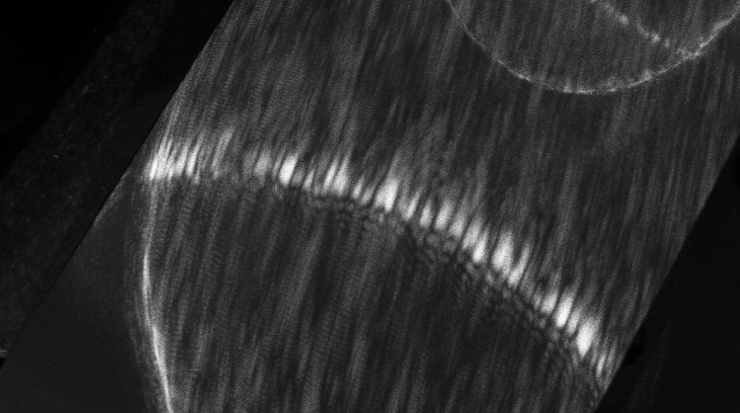
\includegraphics[keepaspectratio,width=15cm]{speckle/figures/Ag_LaSFN9_cone_lens11_cam-8899.jpg}
\caption{A portion of the cone speckle, distorted by a lens and projected on to a piece of paper.}
\label{fig:examplespeckle}
\end{figure}
\section{Introduction}
Under most circumstances, the intensity distribution of light
scattered in to the cone is not spatially homogeneous, but exhibits
distinctive fluctuations known as \textit{speckle}
arising from interference of multiple coherent waves with
statistically random amplitudes and phases.  In optics, speckle is closely
related to the mesoscopic phenomena of universal conductance
fluctuations~\cite{lee1985universal}, and likewise exhibits many of the
same physical phenomena such as coherent
backscattering~\cite{akkermans1986coherent} and the memory
effect~\cite{freund1988memory}.

Speckle is also known to host a wealth of interesting
properties~\cite{goodman1975statistical}~\cite{freund19981001},
particularly in the multiple scattering regime~\cite{feng1986sensitivity}.
Optical speckle in the multiple scattering regime has been shown to be
extraordinary sensitive to both the configuration and
motion~\cite{berkovits1994correlations} of its scatterers.  Indeed, in this
way a speckle pattern may be seen as a unique
``fingerprint''~\cite{ravikanth2001physical} of the underlying scattering
microstructure.  Such principles have been exploited in a diverse set of
applications such as diffusing wave spectroscopy~\cite{pine1988diffusing}
and dynamic light scattering~\cite{berne2000dynamic} in the time domain,
and speckle has been shown to be sensitive to the sub-wavelength
motions~\cite{berkovits1991sensitivity} or
inclusions~\cite{berkovits1990theory} of single scatterers.

As there is no prior work related to cone speckle, this chapter begins with
a discussion of generalized speckle fields.  In particular will look at the
two most important characteristic properties of speckle: size and contrast.  

THIS INTRODUCTION SUCKS!  MAKE IT BETTER!

Static scattering microstructure.

We omit any specific influence of the changes in the underlying scattering
microstructure, a topic reserved for \Chapter{ch:scatteringmicro}.
